\documentclass[twoside,cjk,UTF8]{nputhesis}

\begin{document}
\schoolno{10699}
%\classno{}
%\secretlevel{}
\title[ Binaural Rendering Technology In Augmented Reality ]{	增强现实中\\双耳渲染技术研究}
\author[Jieru Chen]{陈洁茹}
\authorno{2018200480}
\major[Signal and Information Processing]{信号与信息处理}
\supervisor[Wen~Zhang~,~Jingdong~Chen]{张雯~~陈景东}
\applydate[March 2021]{2021~年~3~月}
\support{本文研究得到XX基金(编号:XXXXXXX)资助。}
\makecover

\frontmatter
% 中文摘要
\begin{abstract}
	
	声学场景的双耳渲染旨在给听众提供身临其境的体验,是虚拟现实、增强现实、沉浸式多媒体产品、虚拟声学等领域的重要研究课题。最近,基于球谐分解的双耳渲染算法得到了广泛关注。该算法对声场和头相关传递函数进行球谐函数展开,并且直接在球谐域进行渲染,避免了虚拟扬声器数目和位置对听感的影响。但是此类算法存在声场和头相关传递函数不匹配的问题,例如通常录音设备的尺寸小于人头尺寸,声场分解阶次(通常小于~5~阶)远小于头相关传递函数的分解阶次(34~阶)。这些不匹配问题导致定位线索的损伤、空间感的降低和音色的改变。
	
	本论文主要针对以上问题,从录制声场和头相关传递函数两方面出发,对原始算法加以改进。主要的研究内容包括以下四个方面:
	
	1. 深入研究了基于球谐分解的双耳渲染算法及其存在的问题。对声场和头相关传递函数的球谐分解及系数获取方法进行研究,针对空心球和刚性球展开讨论,给出了正确获取声场系数所需的麦克风数目,以及两种球阵所获取的声场系数的区别。
	
	2. 研究了头相关传递函数的预处理方法,并通过实验验证了该方法的有效性。该方法采用与频率相关的相位对准,保留低频相位信息的同时对高频的相位加以修正。和直接使用最小二乘方法求解头相关传递函数的球谐分量相比,该预处理方法一方面可以准确地表示头相关传递函数的幅度谱,另一方面有效降低了头相关传递函数的分解阶次。
	
	3. 提出了一种声场扩阶理论和一种新的双耳渲染算法。该理论对麦克风阵列的采集声场进行分析,将入射声场分解为直达波和混响场的叠加。根据直达波入射方向进行空间加窗处理,可以实现声场分量的阶次提升,同时扩大控制区域的半径。并且本研究将声场扩阶理论、头相关传递函数预处理和基于球谐分解的双耳渲染算法相结合,实现了基于声场扩阶的双耳渲染算法。
	
	4. 在消声室和混响环境下,从双耳时间差、双耳声级差和双耳听觉互相关系数这三个评价指标出发,将本文所提出的算法与对标算法进行对比和分析,验证本算法的有效性。实验结果表明,在不同的混响情况下、声源位于不同方向时,本文所提出的双耳渲染算法均能达到较好的效果,优于现有算法。并且对空心球和刚性球在不同双耳渲染算法下的性能进行对比,验证了刚性球的优越性。
	
	%\lipsum[2-3]
	\begin{keywords}
		双耳渲染、头相关传递函数、空间音频、球谐分解、声场扩阶
	\end{keywords}
\end{abstract}

% 英文摘要
\begin{Abstract}
	
	Binaural rendering of acoustic scenes aims to provide the audience with an immersive experience. It is an important research topic in the fields of virtual reality, augmented reality, immersive multimedia products, and virtual acoustics. Recently, binaural rendering algorithms based on spherical harmonic decomposition have received much attention. This algorithm performs spherical harmonic expansion of sound field and head-related transfer function(~HRTF~), and renders directly in spherical harmonic domain, avoiding the influence of the number and position of virtual speakers on hearing sense.
	However, there are some mismatches between the sound field and the head-related transfer function in this kind of algorithm. For example, the size of the recording equipment is usually smaller than the head size, and the decomposition order of the sound field (usually less than ~5~ order) is much smaller than the decomposition order of the head-related transfer function (~34~ order). These mismatches lead to impairments of localization cues, loss of spaciousness, and changes in timbre.
	
	Aiming at the above problems, this paper improves the original algorithm from two aspects, sound field and head-related transfer function. The main research contents include the following four aspects:
	
	1. The binaural rendering algorithm based on spherical harmonic decomposition and its problems are studied in detail. The spherical harmonic decomposition and coefficient calculation method of sound field and HRTF are studied, and the number of microphones which is needed to acquire sound field coefficient correctly. The difference of sound field coefficient obtained by open and rigid spherical array are discussed.
	
	2. The preprocessing method of head-related transfer function is studied and the effectiveness of this method is verified by experiments. In this method, the frequency-dependent phase alignment is adopted to retain the phase information of low frequency and modify the phase information of high frequency. Compared with the least square method, this method can not only accurately represent the magnitude spectrum of the head-correlation transfer function, but also effectively reduce the decomposition order of the head-correlation transfer function.
	
	3. A new theory for enlarging the order of sound field and a new binaural rendering algorithm are proposed. In this theory, the incident sound field is decomposed into the superposition of direct component and diffuse field.
	According to the direction of direct component, spatial masking can improve the order of the sound field and enlarge the radius of the control area. In addition,  a new binaural rendering algorithm is realised by combing combines this theory , the frequency-dependent phase alignment preprocessing method of the head-correlation transfer function and the binaural rendering algorithm based on spherical harmonic decomposition.
	
	
	4. In anechoic chamber and reverberation environment, the algorithm proposed in this paper is compared and analyzed from three evaluation indexes , interaural time difference , interaural level difference and interaural cross-correlation. The experimental results show that the binaural rendering algorithm proposed in this paper can achieve better results under different reverberation environments and sound source directions, which is superior to the existing algorithms. The performance of open and rigid spherical array under different binaural rendering algorithms is compared to verify the superiority of rigid ball.
	
	
	\begin{Keywords}
		Binaural rendering, head-related transfer function, spatial audio, spherical harmonic decomposition, sound field amplification
	\end{Keywords}
\end{Abstract}
\tableofcontents

\mainmatter  % 开始各章节
%如果此处include无法成功,将子tex文件的Document的Document setting的 CPconvert的Document Format更改为UTF-8
\chapter{绪论}

\section{研究背景}

以下为一段文字

视频提供了功能强大的方法帮助您证明您的观点。当您单击联机视频时,可以在想要添加的视频的嵌入代码中进行粘贴。您也可以键入一个关键字以联机搜索最适合您的文档的视频。
为使您的文档具有专业外观,提供了页眉、页脚、封面和文本框设计,这些设计可互为补充。例如,您可以添加匹配的封面、页眉和提要栏。单击“插入”,然后从不同库中选择所需元素。
主题和样式也有助于文档保持协调。当您单击设计并选择新的主题时,图片、图表或 SmartArt 图形将会更改以匹配新的主题。当应用样式时,您的标题会进行更改以匹配新的主题。
使用在需要位置出现的新按钮在 Word 中保存时间。若要更改图片适应文档的方式,请单击该图片,图片旁边将会显示布局选项按钮。当处理表格时,单击要添加行或列的位置,然后单击加号。
在新的阅读视图中阅读更加容易。可以折叠文档某些部分并关注所需文本。如果在达到结尾处之前需要停止读取,Word 会记住您的停止位置 - 即使在另一个设备上
\cite{geim_van_2013}。
\subsection{技术应用}
当双耳渲染技术足够成熟时,其应用包括:
\begin{itemize}[leftmargin=*]
\item 提高语言通信的可懂度。目前绝大部分的语言通信采用的是单通路的信号传输系统,不能实现目标语言声源与其他声源在空间上分离,因而语言可懂度会变差。如果引入双耳渲染技术,对原始场景进行重现保留声源的空间信息,就可以提高语言通信的质量;\cite{_fe-p_2020}
\item 引导视觉定位。声音信息的空间化可以引导视觉定位,甚至可以在不借助视觉的情况下寻找目标,从而减少寻找目标以及采取应对措施的时间,提高安全性。主要用途是民用或军用救援搜索、旅游或博物馆向导、盲人的导向和信息系统;\cite{liu_approaching_2018},如图\ref{picexam}所示。
\item 提高语言通信的可懂度。目前绝大部分的语言通信采用的是单通路的信号传输系统,不能实现目标语言声源与其他声源在空间上分离,因而语言可懂度会变差。如果引入双耳渲染技术,对原始场景进行重现保留声源的空间信息,就可以提高语言通信的质量;\cite{_fe-p_2020}
\item 引导视觉定位。声音信息的空间化可以引导视觉定位,甚至可以在不借助视觉的情况下寻找目标,从而减少寻找目标以及采取应对措施的时间,提高安全性。主要用途是民用或军用救援搜索、旅游或博物馆向导、盲人的导向和信息系统;\cite{liu_approaching_2018},如图\ref{picexam}所示。
\item 提高语言通信的可懂度。目前绝大部分的语言通信采用的是单通路的信号传输系统,不能实现目标语言声源与其他声源在空间上分离,因而语言可懂度会变差。如果引入双耳渲染技术,对原始场景进行重现保留声源的空间信息,就可以提高语言通信的质量;\cite{_fe-p_2020}
\item 引导视觉定位。声音信息的空间化可以引导视觉定位,甚至可以在不借助视觉的情况下寻找目标,从而减少寻找目标以及采取应对措施的时间,提高安全性。主要用途是民用或军用救援搜索、旅游或博物馆向导、盲人的导向和信息系统;\cite{liu_approaching_2018},如图\ref{picexam}所示。
\end{itemize}

\section{图片}
视频提供了功能强大的方法帮助您证明您的观点。当您单击联机视频时,可以在想要添加的视频的嵌入代码中进行粘贴。您也可以键入一个关键字以联机搜索最适合您的文档的视频。
为使您的文档具有专业外观,Word 提供了页眉、页脚、封面和文本框设计,这些设计可互为补充。例如,您可以添加匹配的封面、页眉和提要栏。单击“插入”,然后从不同库中选择所需元素。
主题和样式也有助于文档保持协调。当您单击设计并选择新的主题时,图片、图表或 SmartArt 图形将会更改以匹配新的主题。当应用样式时,您的标题会进行更改以匹配新的主题。
使用在需要位置出现的新按钮在 Word 中保存时间。若要更改图片适应文档的方式,请单击该图片,图片旁边将会显示布局选项按钮。当处理表格时,单击要添加行或列的位置,然后单击加号。
在新的阅读视图中阅读更加容易。可以折叠文档某些部分并关注所需文本。如果在达到结尾处之前需要停止读取,Word 会记住您的停止位置 - 即使在另一个设备上
\begin{figure}[H]
	\centering
	
\includegraphics[width=0.6\textwidth]{figure/chapter1/Omni.jpg}
	\caption{不带子图图片示例 }	
	\label{picexam}
\end{figure}
视频提供了功能强大的方法帮助您证明您的观点。当您单击联机视频时,可以在想要添加的视频的嵌入代码中进行粘贴。您也可以键入一个关键字以联机搜索最适合您的文档的视频。
为使您的文档具有专业外观,Word 提供了页眉、页脚、封面和文本框设计,这些设计可互为补充。例如,您可以添加匹配的封面、页眉和提要栏。单击“插入”,然后从不同库中选择所需元素。
主题和样式也有助于文档保持协调。当您单击设计并选择新的主题时,图片、图表或 SmartArt 图形将会更改以匹配新的主题。当应用样式时,您的标题会进行更改以匹配新的主题。
使用在需要位置出现的新按钮在 Word 中保存时间。若要更改图片适应文档的方式,请单击该图片,图片旁边将会显示布局选项按钮。当处理表格时,单击要添加行或列的位置,然后单击加号。
在新的阅读视图中阅读更加容易。可以折叠文档某些部分并关注所需文本。如果在达到结尾处之前需要停止读取,Word 会记住您的停止位置 - 即使在另一个设备上yekeyi

\begin{figure}[H]
\centering
\subfigure[]{

\includegraphics[width=0.21\textwidth]{figure/chapter1/Omni.jpg}}
\subfigure[]{

\includegraphics[width=0.21\textwidth]{figure/chapter1/Omni.jpg}}\\
\subfigure[]{

\includegraphics[width=0.21\textwidth]{figure/chapter1/Omni.jpg}}
\hspace{3cm}
\subfigure[]{

\includegraphics[width=0.21\textwidth]{figure/chapter1/Omni.jpg}}

\caption{带子图图片示例,(a)1,(b)2,(c)3,(d)4}
\label{fig:binaural_recording}
\end{figure}

视频提供了功能强大的方法帮助您证明您的观点。当您单击联机视频时,可以在想要添加的视频的嵌入代码中进行粘贴。您也可以键入一个关键字以联机搜索最适合您的文档的视频。
为使您的文档具有专业外观,Word 提供了页眉、页脚、封面和文本框设计,这些设计可互为补充。例如,您可以添加匹配的封面、页眉和提要栏。单击“插入”,然后从不同库中选择所需元素。
主题和样式也有助于文档保持协调。当您单击设计并选择新的主题时,图片、图表或 SmartArt 图形将会更改以匹配新的主题。当应用样式时,您的标题会进行更改以匹配新的主题。

\section{表格}
\begin{tabular}{ccc}
	&  &  \\
	&  &  \\
\end{tabular}
\begin{table}[H]
\caption{HRTF 预处理方法}
\centering
\begin{tabular}{|c|c|c|}
\hline
方法 & 预处理对象 & 预处理方法 \\
\hline
$H_{a}$ & 复频谱 & 时间对准 \\
$H_{s m}$ & \multicolumn{1}{l|}{复频谱} & 平滑 \\
$|H|$ & 幅度谱 & 无 \\

\hline
\end{tabular}
\end{table}
视频提供了功能强大的方法帮助您证明您的观点。当您单击联机视频时,可以在想要添加的视频的嵌入代码中进行粘贴。您也可以键入一个关键字以联机搜索最适合您的文档的视频。
为使您的文档具有专业外观,Word 提供了页眉、页脚、封面和文本框设计,这些设计可互为补充。例如,您可以添加匹配的封面、页眉和提要栏。单击“插入”,然后从不同库中选择所需元素。
主题和样式也有助于文档保持协调。当您单击设计并选择新的主题时,图片、图表或 SmartArt 图形将会更改以匹配新的主题。当应用样式时,您的标题会进行更改以匹配新的主题。
\subsection{三线表}
\begin{table}[H]
	\caption{HRTF 预处理方法}
	\centering
	\begin{tabular*}{\hsize}{@{\extracolsep{\fill}}ccc}
		\toprule
		方法 & 预处理对象 & 预处理方法 \\
		\midrule
		$H_{a}$ & 复频谱 & 时间对准 \\
		$H_{s m}$ & 复频谱 & 平滑 \\
		$|H|$ & 幅度谱 & 无 \\
		\bottomrule
	\end{tabular*}
	\label{tab.pre_processing}
\end{table}
视频提供了功能强大的方法帮助您证明您的观点。当您单击联机视频时,可以在想要添加的视频的嵌入代码中进行粘贴。您也可以键入一个关键字以联机搜索最适合您的文档的视频。
为使您的文档具有专业外观,Word 提供了页眉、页脚、封面和文本框设计,这些设计可互为补充。例如,您可以添加匹配的封面、页眉和提要栏。单击“插入”,然后从不同库中选择所需元素。
主题和样式也有助于文档保持协调。当您单击设计并选择新的主题时,图片、图表或 SmartArt 图形将会更改以匹配新的主题。当应用样式时,您的标题会进行更改以匹配新的主题。
\begin{table}[htbp]
	\centering
	\caption{主要仪器设备}
	\label{instruments}
	\renewcommand\arraystretch{1.5}
	\zihao{5}
	\begin{tabular*}{\hsize}{@{}@{\extracolsep{\fill}}ccc@{}}
		\toprule
		仪器名称          &      型号       &      生产厂家      \\ 
		\midrule
		超纯水系统         &   CSR-1-10    & 北京爱斯泰克科技开发有限公司 \\
		电热恒温鼓风干燥箱     &   DGG-9030B   &  上海森信实验仪器有限公司  \\
		分析天平          &    AUW220D    &    日本岛津制作所     \\
		程序升温箱式炉       &   KSL 1200X   &   合肥科晶材料有限公司   \\
		恒温加热磁力搅拌器     &     CL-4      &  巩义市予华仪器有限公司   \\
		程序升温管式炉       &    KSL YDL    &   扬州宝鼎电热电器厂    \\
		X射线衍射分析仪      &  X’pert pro   &    日本Rigaku    \\
		场发射扫描电子显微镜    &   JSM-7001F   & 日本电子株式会社(JEOL) \\
		紫外可见分光光度计     &   UV-9000S    &   上海元析仪器有限公司   \\
		%		  & 	Escalab 250Xi & 赛默飞世尔科技公司\\
		离心机          &    TDL-6A     & 上海菲恰尔分析仪器有限公司  \\
		\bottomrule
	\end{tabular*}
\end{table}
视频提供了功能强大的方法帮助您证明您的观点。当您单击联机视频时,可以在想要添加的视频的嵌入代码中进行粘贴。您也可以键入一个关键字以联机搜索最适合您的文档的视频。
为使您的文档具有专业外观,Word 提供了页眉、页脚、封面和文本框设计,这些设计可互为补充。例如,您可以添加匹配的封面、页眉和提要栏。单击“插入”,然后从不同库中选择所需元素。
主题和样式也有助于文档保持协调。当您单击设计并选择新的主题时,图片、图表或 SmartArt 图形将会更改以匹配新的主题。当应用样式时,您的标题会进行更改以匹配新的主题。视频提供了功能强大的方法帮助您证明您的观点。当您单击联机视频时,可以在想要添加的视频的嵌入代码中进行粘贴。您也可以键入一个关键字以联机搜索最适合您的文档的视频。
为使您的文档具有专业外观,Word 提供了页眉、页脚、封面和文本框设计,这些设计可互为补充。例如,您可以添加匹配的封面、页眉和提要栏。单击“插入”,然后从不同库中选择所需元素。
主题和样式也有助于文档保持协调。当您单击设计并选择新的主题时,图片、图表或 SmartArt 图形将会更改以匹配新的主题。当应用样式时,您的标题会进行更改以匹配新的主题。视频提供了功能强大的方法帮助您证明您的观点。当您单击联机视频时,可以在想要添加的视频的嵌入代码中进行粘贴。您也可以键入一个关键字以联机搜索最适合您的文档的视频。
为使您的文档具有专业外观,Word 提供了页眉、页脚、封面和文本框设计,这些设计可互为补充。例如,您可以添加匹配的封面、页眉和提要栏。单击“插入”,然后从不同库中选择所需元素。
主题和样式也有助于文档保持协调。当您单击设计并选择新的主题时,图片、图表或 SmartArt 图形将会更改以匹配新的主题。当应用样式时,您的标题会进行更改以匹配新的主题。

\begin{table*}
	\centering
	\caption{Comparison of different obfuscations in terms of their transformation capabilities}
	\begin{tabular}{ccccc} % 控制表格的格式
		\toprule
		\multirow{2}{*}{Obfuscators} & \multicolumn{4}{c}{Transformations}   \\
		\cline{2-5}  % 这部分是画一条横线在2-6 排之间
		&    Renaming & Dead code removal & control flow obfuscation & string encryption \\
		\midrule
		Proguard &  \checkmark & $\times$  & $\times$ & \checkmark   \\
		Allatori & \checkmark & $\times$  & $\times$ & \checkmark \\
		DashO & \checkmark & $\times$  & $\times$ & \checkmark \\
		Androcrypt & \checkmark & $\times$  & $\times$ & \checkmark  \\
		\bottomrule
	\end{tabular}
	\label{tbl:table1}
\end{table*}


\section{公式}
从~SOFA~格式角度定义到最终角度定义的转换公式为:
\[
M=
\left[
\begin{matrix}
	\textcolor{red}{\varepsilon_{11}} & \varepsilon_{12} & \varepsilon_{13}\\
	\varepsilon_{21} & \varepsilon_{22} & \varepsilon_{23}\\
	\varepsilon_{31} & \varepsilon_{32} & \varepsilon_{33}\\
\end{matrix}\right]
\]

\begin{align}
	\label{111}
	\phi & = \text{mod}~\left( 360^{\circ}-\varphi_{\text{SOFA}}, 360^{\circ} \right)  \nonumber \\
	\theta & =  90^{\circ} - \theta_{\text{SOFA}} 	
\end{align}

\[
\mu = \frac{B}{H}=\frac{B_0 e^{i\omega t-\delta}}{H_0 e^{i\omega t}}=\frac{B_0}{H_0}\cos\delta-i\frac{B_0}{H_0}\sin\delta
\]
其中,mod~表示取余。详见 式\ref{111}
\begin{equation}
\eta = \frac{qVN_0}{d^2}\left\{(\mu\tau)_e \left[1-\text{exp}\left(\frac{x_0-d}{\frac{(\mu\tau)_e V}{d}}\right)\right]+(\mu\tau)_h \left[1-\text{exp}\left(\frac{-x_0}{\frac{(\mu\tau)_h V}{d}}\right)\right]\right\}
\end{equation}

\chapter{示例}
\label{chp:example}
本部分为列表、表格、图片等示例
\section{列表示例}
\begin{itemize}[leftmargin=*]
	\item 这是一个列表项目
	\item 这是一个列表项目
	\item 这是一个列表项目
	\item 这是一个列表项目
	\item 这是一个列表项目
\end{itemize}
\section{引用示例}
\label{sec:ref}
文档的各个部分引用前均需采用 \textbackslash label 命令添加标签,图表公式添加在环境内部,所需引用章节添加于命令之后,建议对不同类型label 命名时进行区分。

参考文献引用:\cite{liu_approaching_2018},图片引用:如图 \ref{picexam}所示,表格引用:如表\ref{tbl:pre_processing}所示,公式引用:如式(\ref{eq:111})所示,章节引用:第 \ref{chp:example}章、第  \ref{sec:ref}节、第 \ref{ssec:pic}节。

\section{图片}
论文中的图片插入通常在一下方式中选择一种即可,每次插入可以拷贝一份粘贴至目标位置,并更改路径、大小、标题和label。
\subsection{无子图图片}
通常来说,论文中的图片插入时只有一个文件,子图应在外部拼接好后导出为一整张图片,再进行导入,并且由于材料学院双语标题要求,采用\textbackslash bicaption{中文}{英文}实现,前者为中文,后者为英文。如不需要双语标题,改为\textbackslash caption{标题}即可。
\label{ssec:pic}
\begin{figure}[H]
	\centering
	
\includegraphics[width=0.6\textwidth]{figure/chapter1/Omni.jpg}%设置图片宽度和源文件路径,无命名冲突时可不包含文件类型后缀
	\bicaption{不带子图图片示例,(a)1,(b)2,(c)3,(d)4}{This is an english title}% 双语标题
	\label{picexam}%标签
\end{figure}

\begin{figure}[H]
	\centering
	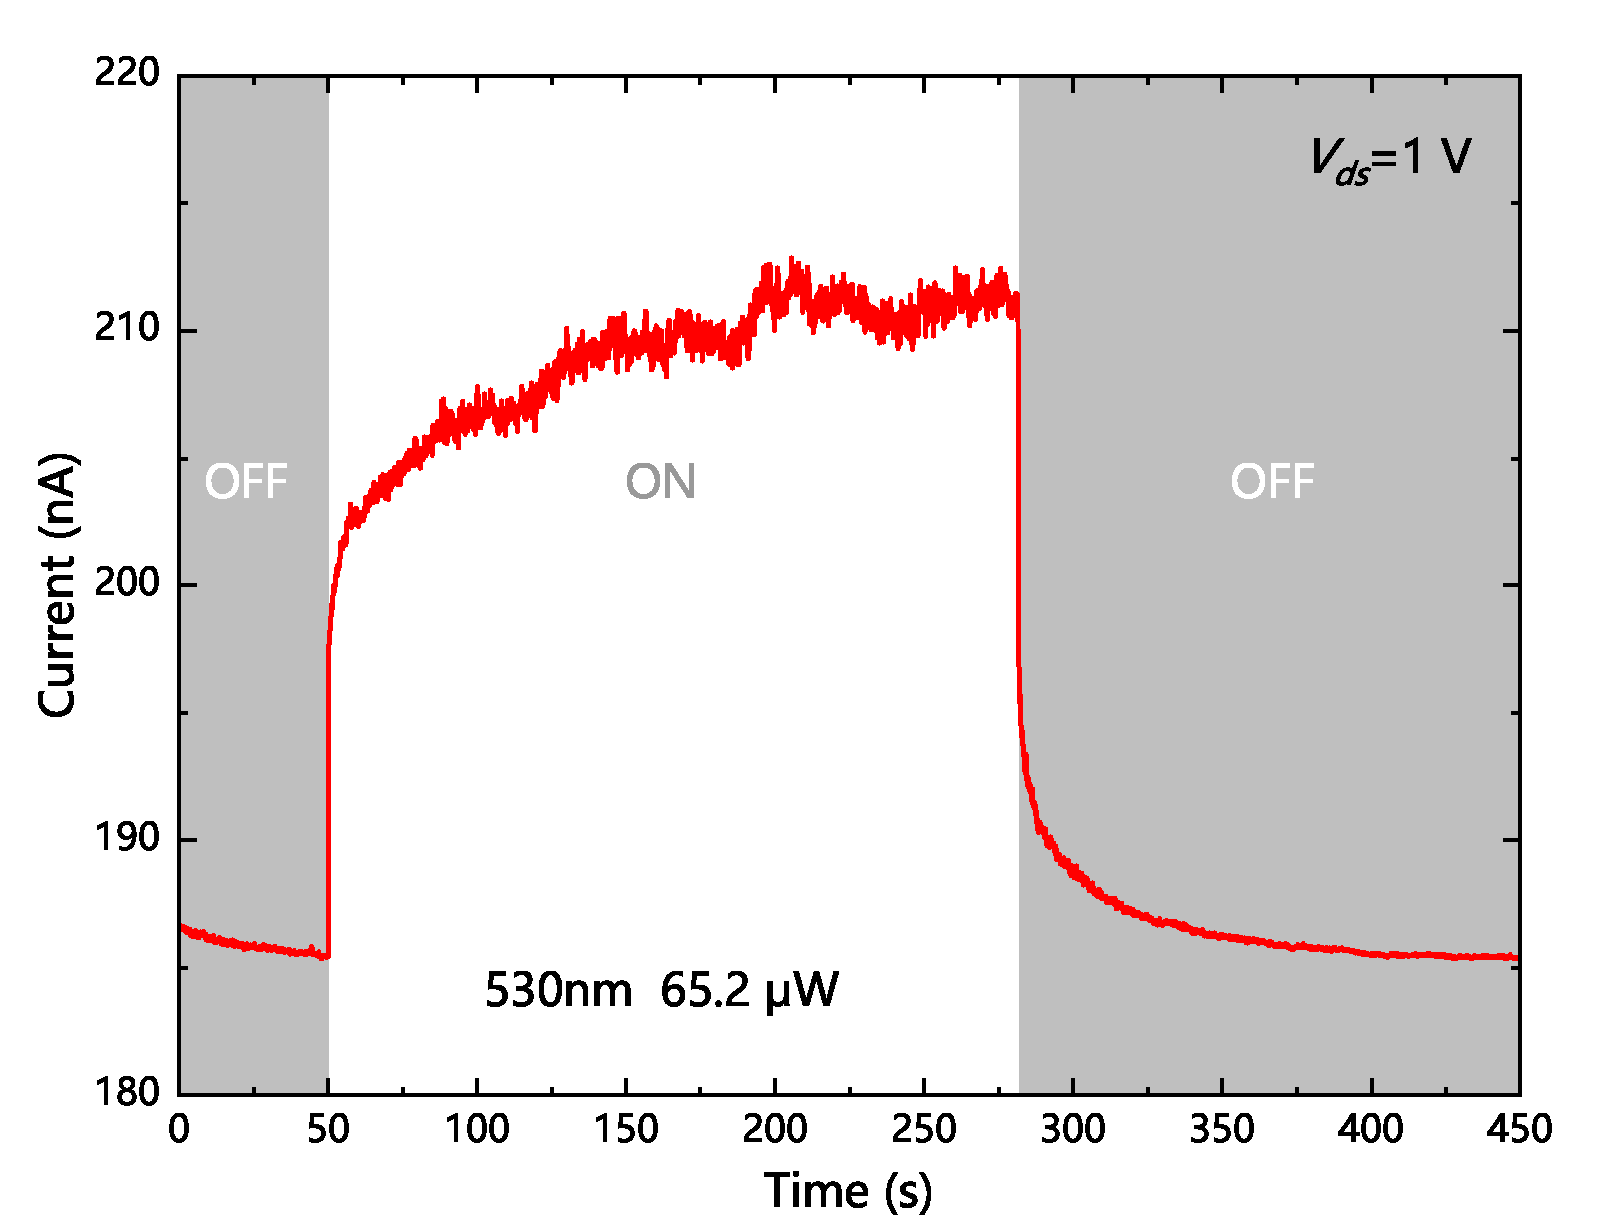
\includegraphics[width=0.6\textwidth]{figure/chapter1/Graph3.pdf}
	\caption{矢量图片示例,无英文标题}	
	\label{pdfpic}
\end{figure}
\subsection{带有子图图片}
如坚持使用子图插入的类型,可以采用如下格式:
\begin{figure}[H]
	\centering
	\subfigure[]{
		
\includegraphics[width=0.21\textwidth]{figure/chapter1/Omni.jpg}}
	\subfigure[]{
		
\includegraphics[width=0.21\textwidth]{figure/chapter1/Omni.jpg}}\\%分行
	\subfigure[]{
		
\includegraphics[width=0.21\textwidth]{figure/chapter1/Omni.jpg}}
	\hspace{3cm}
	\subfigure[]{
		
\includegraphics[width=0.21\textwidth]{figure/chapter1/Omni.jpg}}
	
	\bicaption{带子图图片示例,(a)1,(b)2,(c)3,(d)4}{This is an english figure title}
	\label{fig:binaural_recording}
\end{figure}

视频提供了功能强大的方法帮助您证明您的观点。当您单击联机视频时,可以在想要添加的视频的嵌入代码中进行粘贴。您也可以键入一个关键字以联机搜索最适合您的文档的视频。
为使您的文档具有专业外观,Word 提供了页眉、页脚、封面和文本框设计,这些设计可互为补充。例如,您可以添加匹配的封面、页眉和提要栏。单击“插入”,然后从不同库中选择所需元素。
主题和样式也有助于文档保持协调。当您单击设计并选择新的主题时,图片、图表或 SmartArt 图形将会更改以匹配新的主题。当应用样式时,您的标题会进行更改以匹配新的主题。

\section{表格}
表格与图片类似,但表格和图片独立编号,且标题在上。一般来说论文中应采用三线表,但为了应对特殊需求,以下仍给出普通表格示例:
\subsection{普通表格}
\begin{table}[H]
	\caption{HRTF 预处理方法}
	\centering
	\begin{tabular}{|c|c|c|}
		\hline
		方法 & 预处理对象 & 预处理方法 \\
		\hline
		$H_{a}$ & 复频谱 & 时间对准 \\
		$H_{s m}$ & \multicolumn{1}{l|}{复频谱} & 平滑 \\
		$|H|$ & 幅度谱 & 无 \\
		
		\hline
	\end{tabular}
\end{table}

\subsection{三线表}
三线表示例如下,\textbackslash toprule 和 \textbackslash bottomrule为粗线,\textbackslash midrule为细线,toprule和midrule之间应为表格标题行。
\begin{table}[H]
	\bicaption{HRTF 预处理方法}{ HRTF pre-process mothod}
	\centering
	\begin{tabular*}{\hsize}{@{\extracolsep{\fill}}ccc}
		\toprule
		方法 & 预处理对象 & 预处理方法 \\
		\midrule
		$H_{a}$ & 复频谱 & 时间对准 \\
		$H_{s m}$ & 复频谱 & 平滑 \\
		$|H|$ & 幅度谱 & 无 \\
		\bottomrule
	\end{tabular*}
	\label{tbl:pre_processing}
\end{table}



\begin{table}[htbp]
	\centering
	\caption{Comparison of different obfuscations in terms of their transformation capabilities}
	\begin{tabular}{ccccc} % 控制表格的格式
		\toprule
		\multirow{2}{*}{Obfuscators} & \multicolumn{4}{c}{Transformations}   \\
		\cline{2-5}  % 这部分是画一条横线在2-6 排之间
		&    Renaming & Dead code removal & control flow obfuscation & string encryption \\
		\midrule
		Proguard &  \checkmark & $\times$  & $\times$ & \checkmark   \\
		Allatori & \checkmark & $\times$  & $\times$ & \checkmark \\
		DashO & \checkmark & $\times$  & $\times$ & \checkmark \\
		Androcrypt & \checkmark & $\times$  & $\times$ & \checkmark  \\
		\bottomrule
	\end{tabular}
	\label{tbl:table1}
\end{table}

\section{公式}
公式示例如下:

不带编号公式:
\[
M=
\left[
\begin{matrix}
	\textcolor{red}{\varepsilon_{11}} & \varepsilon_{12} & \varepsilon_{13}\\
	\varepsilon_{21} & \varepsilon_{22} & \varepsilon_{23}\\
	\varepsilon_{31} & \varepsilon_{32} & \varepsilon_{33}\\
\end{matrix}\right]
\]
\[
\mu = \frac{B}{H}=\frac{B_0 e^{i\omega t-\delta}}{H_0 e^{i\omega t}}=\frac{B_0}{H_0}\cos\delta-i\frac{B_0}{H_0}\sin\delta
\]

带编号公式:
\begin{equation}
	\eta = \frac{qVN_0}{d^2}\left\{(\mu\tau)_e \left[1-\text{exp}\left(\frac{x_0-d}{\frac{(\mu\tau)_e V}{d}}\right)\right]+(\mu\tau)_h \left[1-\text{exp}\left(\frac{-x_0}{\frac{(\mu\tau)_h V}{d}}\right)\right]\right\}
\end{equation}

多行带编号公式:
\begin{align}
	\label{eq:111}
	\phi & = \text{mod}~\left( 360^{\circ}-\varphi_{\text{SOFA}}, 360^{\circ} \right)  \nonumber \\
	\theta & =  90^{\circ} - \theta_{\text{SOFA}} 	
\end{align}





\backmatter % 参考文献之前
\bibliographystyle{nputhesis}
\bibliography{refs}
% 如果参考文献中有&需要展示,应该使用\&

%附录为可选项
%\Appendix

\Thanks

时光飞逝,转眼间已经要说再见,在西工大度过的七年时光历历在目,有着太多的不舍。学习和成长的过程,离不开老师的悉心教导和同学的关心帮助,在此我要向大家表示我最真诚的感谢。

首先要特别感谢我的两位指导老师:张雯教授和陈景东教授。从论文选题到研究工作的开展以及论文的撰写,都是在两位老师的指导下进行的。两位老师认真负责、精益求精的工作态度、渊博的知识储备、平易近人的处事方法深深影响了我,永远是我科研和生活的人生榜样。从本科毕业设计到现在,这三年多的时间里,我从刚开始的科研小白到现在有一定的理解和成果,都离不开两位老师的耐心指导,一次次的讨论让我对自己的研究方向和工作内容有了清晰的认知,使我的学习能力与动手能力得到了提升。老师们不仅在科研上给予帮助,还非常关心我们的生活情况和就业进展。

感谢教研室的师兄师姐和师弟师妹们,他们在整个研究生生涯中给予了我很多帮助,一起度过了很多快乐的时光。在探讨交流过程中,我吸收了很多宝贵的经验,为科研工作奠定基础。其中特别感谢郗经纬同学,在遇到问题时共同讨论、互帮互助,还有同级的陈奕彤和李梦真,在整个论文的撰写过程中相互鼓励,正是这种合作精神,给我们的研究生生涯画上了一个完美的句号。感谢张俊卿师兄在我遇到不懂的问题时给予分析和建议,对论文提出修改意见,同时感谢帮我审阅论文的师妹尤新雅、胡轩琦、师弟王佳乐,感谢你们提出的宝贵意见。感谢我硕士期间的宝藏舍友们,每天回到宿舍都会有一个开心轻松的氛围,互相关心,相信我们七年的友谊在之后的时间里可以得到更好的发展。

在此,还要感谢我的家人和男朋友对我无微不至的关心与理解。你们是我的坚强后盾,对我的任何决定都给予支持,让我可以毫无顾虑地勇往直前。在我遇到困难和压力时,你们的陪伴和鼓励使我能够保持乐观的心态,做出更好的成绩。

同时,我还要感谢我的班主任李道江老师和就业指导中心这个大家庭,在我的生涯规划和求职过程中给予指导和关心。最后还要向本领域进行相关研究的学者专家,以及各位审阅评议论文的老师表示由衷的感谢!

\Work

\noindent
\textbf{发表学术论文}
\begin{enumerate}
	\renewcommand{\labelenumi}{[\theenumi]}
	\item Chen J, Dou S, Zhang W. Binaural rendering based on linear differential microphone array and ambisonic reproduction[J]. Journal of Fudan University(Natural Science),2019, 58(3):370–377.
\end{enumerate}

~\\

\noindent
\textbf{发表专利}
\begin{enumerate}
	\renewcommand{\labelenumi}{[\theenumi]}
	\item 专利名称:一种混合型主动降噪方法与系统(已受理,第一发明人)。
	\item 专利名称:一种主动降噪耳机的滤波器设计方法(已受理)。
\end{enumerate}
\statement
%\end{CJK} % 保证中文格式的pdf书签
\end{document}